\documentclass[11pt,a4paper]{article}

\usepackage[utf8]{inputenc}
\usepackage[T1]{fontenc}
\usepackage[english]{babel}
\usepackage{geometry}
\usepackage{microtype}
\usepackage{booktabs}
\usepackage{enumitem}
\usepackage{graphicx}
\usepackage{tikz}
\usetikzlibrary{positioning, shapes.geometric, arrows.meta, backgrounds, fit}
\usepackage{hyperref}

\geometry{margin=2.6cm}
\setlist{noitemsep,topsep=2pt}

\hypersetup{
    colorlinks=true,
    linkcolor=blue,
    filecolor=magenta,      
    urlcolor=blue,
    pdftitle={Research Project Proposal - Davide Ditolve},
    pdfpagemode=FullScreen,
}

\begin{document}

% ------------------------------------------------------------------------------
% 1) FRONTISPIECE
% ------------------------------------------------------------------------------
\section{Frontispiece}

\begin{center}
    
\includegraphics[width=0.22\textwidth]{logo_ecampus.png}\\[0.4cm]
    {\large \textsc{eCampus Telematic University}}\\[0.1cm]
    {\small PhD Program in Applied Sciences to Well-being and Sustainability (XLII Cycle)}\\[0.6cm]
    
    {\large \textbf{RESEARCH PROJECT PROPOSAL}}\\[0.3cm]
    {\Large \textbf{PsyCare-AI: Local AI and Nosographical Grounding for\\ Transparent, Sustainable Clinical Support}}\\[0.8cm]
\end{center}

\noindent
\textbf{Candidate:} Davide Ditolve \hfill \textbf{Research Line:} Research Line 4 - New therapeutic and rehabilitative approaches for health and well-being\\
\textbf{Proposed Supervisor:} Prof. Riccardo Pecori (IINF-05/A)\\[0.4cm]

\subsection*{Abstract}
When a clinician faces a complex case, the need is not for one more automatic answer, but for support that makes its sources and uncertainty visible. The PsyCare-AI proposal is a clinical decision support system (CDSS) designed not as a passive RAG to look for patient information, but as an interactive support, assisting mental health experts directly even during therapeutic sessions, combining LLMs and Agentic workflows grounded in ICD-11 and DSM-5-TR. 
Although AI is at the center, it has no autonomous diagnostic role. Instead, the project explores whether this tool reduces diagnostic oversights and cognitive overload compared to manual consultation. At the same time, it will introduce a ``digital anamnesis'' protocol to include the spontaneous use of chatbots by patients in clinical dialog and examine its associations with well-being and therapeutic alliance. The work combines technical development, an intensive study with clinicians, an observational patient study, and action research in services. Clinical data will be processed leveraging local hardware. In case resources are insufficient, they will be processed via a secure cloud fallback with end-to-end encryption and PII isolation. Cloud resources will support intensive workloads on a huge amount of anonymized data. The final goal is not to automate diagnosis, but to provide a ``Swiss Army knife'' of opportunities for the clinician to tackle any case, reduce cognitive biases, and improve therapeutic support.

\vspace{0.4cm}
\noindent \textbf{Keywords:} Decision Support; Local RAG; Optimized Language Models; Psychophysical Well-being; Sustainability of Care; Digital Anamnesis.

\newpage

% ------------------------------------------------------------------------------
% 2) THEORETICAL INTRODUCTION
% ------------------------------------------------------------------------------
\section{Theoretical introduction}

Promoting the well-being of individuals with psychiatric conditions requires personalized, secure, and sustainable care models. In this context, e-health and clinical decision support systems (CDSS) can offer concrete help, especially when the clinician has to integrate a lot of information in a short time. However, integrating these technologies into psychopathology presents unique clinical, ethical, and technical challenges that prevent their uncritical transposition from general medicine (Cremaschi \& Pierotti, 2026).

Unlike general medicine, which is supported by biological markers, psychopathology is grounded in a clinical object that is subjective, narrative, and relational (Jaspers, 1963; Stanghellini \& Fuchs, 2013). Suffering is expressed through narrative and clinical setting dynamics (Parnas et al., 2013). Deploying Large Language Models (LLMs) to support clinical reasoning introduces critical engineering and well-being challenges:

Differential diagnosis is particularly difficult in ``borderline'' cases: subthreshold presentations, comorbidity, or cases in which similar symptoms point to different categories. Here, borderline does not refer only to borderline personality disorder, but to any presentation with high nosographical ambiguity. The danger lies not strictly in omitting a diagnostic criterion, but in premature closure, anchoring on the initial assumptions, or relying on ambigous findings as confirmation. An LLM can be helpful only if it does not exclude any hypotheses, displays supporting and contradictory evidence, identifies missing information, and proposes new approaches to a question; the ultimate clinical diagnosis remains the clinician's responsibility.

\begin{enumerate}[label=\alph*)]
    \item \textbf{Taxonomic grounding and cognitive bias mitigation:} Gen-AI systems can produce hallucinations and sycophantic responses toward user hypotheses (\textit{sycophancy}; Sharma et al., 2023), with the risk of reinforcing premature diagnostic readings. As analyzed by Vidotto, Ditolve, and Panzeri (2026), LLMs simulate understanding without real semantic intent (the ``epistemology of simulation''). To safeguard patient well-being, the technology is designed not as a standalone tool for patients, but as an interactive co-pilot that assists the clinician during therapeutic sessions, remaining a guidance tool and not a diagnostic authority. From a technical perspective, this requires Retrieval-Augmented Generation (RAG) models trained and grounded to provide outputs based on official taxonomies such as ICD-11 and DSM-5-TR (Cremaschi et al., 2025).
    
    \item \textbf{Data sovereignty and hybrid cloud-edge architectures:} Handling highly confidential patient data requires strict adherence to privacy regulations (e.g. GDPR). Submitting patient records to commercial web-exposed APIs raises the risks of data leakage and loss of control over the data. Thus, designing on-premises solutions, resource-constrained AI architectures is a priority (\textit{pervasive and resource-constrained AI}; Pecori, 2023). Memory and computational capacity can be limiting factors; therefore, the project studies a hybrid cloud-edge architecture: clinical inference runs on local devices or, if the hardware is not enough, on dedicated encrypted cloud nodes. Cloud resources can also handle large-scale model training, fine-tuning, and embedding optimization on datasets.
    
    \item \textbf{The relational dimension and AI as the ``third in the room'':} Patients have shown an increase in commercial chatbots usage as therapeutic surrogates (Cremaschi \& Pierotti, 2026). Such unregulated engagement can lead to cyberchondria, dependency, or isolation (Dohnány et al., 2026). Therefore, it appears vital to bridge this digital experience within the therapeutic relationship by introducing a structured ``digital anamnesis'' protocol, extracting valuable clinical data points from their interactions.
\end{enumerate}

% ------------------------------------------------------------------------------
% 3) RESEARCH OBJECTIVES AND HYPOTHESES
% ------------------------------------------------------------------------------
\section{Research objectives and hypotheses}

The primary question is straightforward: can a local system grounded in traceable nosographical sources help clinicians reduce omissions without increasing mental workload? A second question concerns what is often left outside the consultation: how does chatbot use enter the patient's story and therapeutic relationship?

\subsection{Synergy between Technology and Well-being}

In this project, computer engineering solutions are specifically designed as a co-pilot for the clinician during therapeutic sessions, aiming to support patient psychophysical well-being and facilitate the creation of targeted clinical pathways:
\begin{itemize}
    \item \textbf{Clinical reliability for targeted therapeutic pathways:} Reduce diagnostic omissions and premature closure via the RAG pipeline, enabling clinicians to design targeted, personalized therapeutic pathways early on and minimizing the risk of inappropriate treatments.
    \item \textbf{Software security and data protection:} Protect sensitive patient information by running LLMs at the edge, minimizing data leakage risks.
    \item \textbf{Digital Anamnesis and therapeutic alliance:} Integrate patients' digital habits into the clinical dynamic, transforming their chatbot interactions into valuable insights that protect the therapeutic alliance and promote well-being.
\end{itemize}

\subsection{Specific Objectives}

\begin{enumerate}
    \item \textbf{Designing the decision support system (CDSS):} Engineer a clinician-facing software framework to support real-time therapeutic sessions, driven by edge-based agentic workflows and integrating standard clinical taxonomies in a hybrid edge-cloud setup with secure failover.
    \item \textbf{Clinical-relational study for well-being:} Design and validate a ``digital anamnesis'' protocol to integrate patient AI interactions into clinical practice, focusing on therapeutic pathways and assessing its association with therapeutic alliance.
    \item \textbf{Experimental evaluation:} Measure differential-diagnosis outcomes and quality, unsupported assumptions, diagnostic criteria omissions, cognitive burden, and computational metrics.
    \item \textbf{Governance and Data Privacy guidelines:} Enstablish common recommendations for safe AI adoption in mental health services, compliant with EU regulations.
\end{enumerate}

\subsection{Research Hypotheses}

\begin{itemize}
    \item \textbf{H1 (primary hypothesis):} In contrast to traditional consultation, the CDSS is expected to improve differential-diagnosis completeness, defined as the capacity to identify clinically valid alternatives, even with conflicting or missing data, while investigating unfounded assumptions. Accuracy and NASA-TLX scores will serve as secondary outcomes.
    \item \textbf{H2 (Clinical-Relational Alliance):} Patients with a dysfunctional or compulsive chatbot usage profile (Independent Variable, measured within the Digital Anamnesis) may show lower therapeutic alliance scores (WAI rated by both patient and clinician) and greater baseline symptom severity (BDI-II, BAI) (Dependent Variables) compared to patients with regulated or no chatbot usage.
    \item \textbf{H3 (Efficiency and Sustainability):} Model quantization will open unlock low-cost hardware execution scenarios, with a measurable trade-off between latency and quality. Acceptance baselines will be defined a priori, strictly according to the specific deployment scenario.
\end{itemize}

% ------------------------------------------------------------------------------
% 4) METHODOLOGY
% ------------------------------------------------------------------------------
\section{Methodology}

This study leverages an interdisciplinary mixed-methods research approach, integrating computer engineering for system development, and a clinical-experimental branch to assess the ultimate effect on patient well-being.

\subsection{Study Type and Experimental Design}

\begin{itemize}
    \item \textbf{CDSS Evaluation (Phase 1):} Controlled within-subjects crossover trials using vignettes with different complexities (symptoms, comorbidity, overlap). Order is counterbalanced. Blinded experts will define plausible diagnoses and necessary further inquiries.
    \item \textbf{Observational Study on the Relationship (Phase 2):} A preliminary pilot correlational study involving active patients. Experts will evaluate the Digital Anamnesis for content validity, followed by preliminary assessment of readability, reliability, and convergence. Identified correlations will be considered strictly non-causal.
    \item \textbf{Action Research on Care Quality (Phase 3):} Focus groups with healthcare workers to identify barriers to adoption and define organizational sustainability metrics.
\end{itemize}

\begin{figure}[htbp]
    \centering
    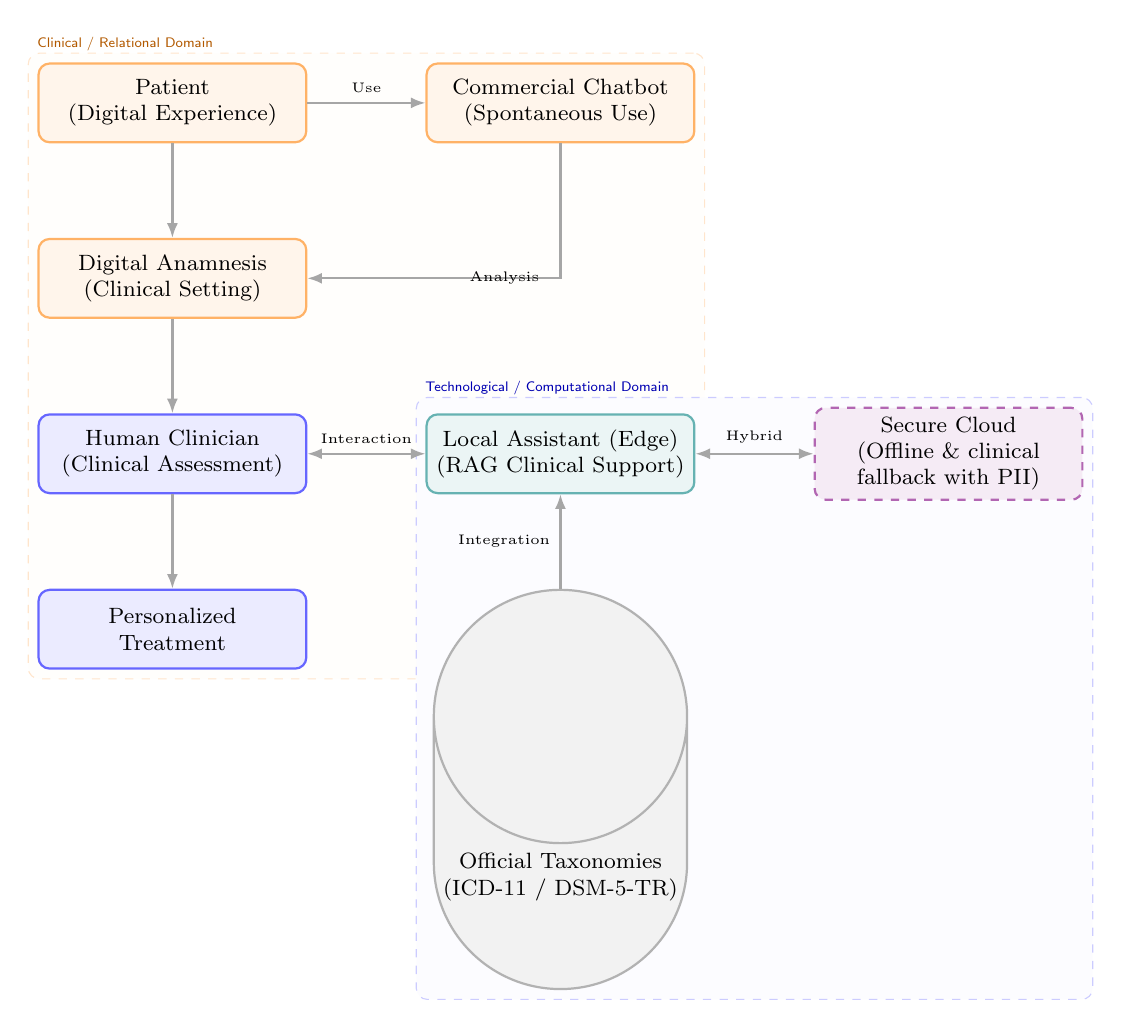
\begin{tikzpicture}[
        node distance=1.2cm and 1.5cm,
        patient_node/.style={draw, rectangle, rounded corners=4pt, minimum width=3.4cm, minimum height=1.0cm, align=center, fill=orange!8, draw=orange!60, thick, font=\footnotesize},
        clinician_node/.style={draw, rectangle, rounded corners=4pt, minimum width=3.4cm, minimum height=1.0cm, align=center, fill=blue!8, draw=blue!60, thick, font=\footnotesize},
        tech_edge_node/.style={draw, rectangle, rounded corners=4pt, minimum width=3.4cm, minimum height=1.0cm, align=center, fill=teal!8, draw=teal!60, thick, font=\footnotesize},
        tech_cloud_node/.style={draw, rectangle, rounded corners=4pt, minimum width=3.4cm, minimum height=1.0cm, align=center, fill=violet!8, draw=violet!60, thick, dashed, font=\footnotesize},
        database_node/.style={draw, cylinder, shape border rotate=90, minimum width=2.4cm, minimum height=1.0cm, align=center, fill=gray!10, draw=gray!60, thick, font=\footnotesize},
        arrow/.style={-{Latex[scale=0.8]}, thick, draw=gray!70},
        bi_arrow/.style={<->, {Latex[scale=0.8]}-{Latex[scale=0.8]}, thick, draw=gray!70}
    ]
        % Nodes
        \node (patient) [patient_node] {Patient\\(Digital Experience)};
        \node (chatbot) [patient_node, right=of patient] {Commercial Chatbot\\(Spontaneous Use)};
        \node (anamnesis) [patient_node, below=of patient] {Digital Anamnesis\\(Clinical Setting)};
        \node (clinician) [clinician_node, below=of anamnesis] {Human Clinician\\(Clinical Assessment)};
        \node (support) [tech_edge_node, right=of clinician] {Local Assistant (Edge)\\(RAG Clinical Support)};
        \node (cloud) [tech_cloud_node, right=of support] {Secure Cloud\\(Offline \& clinical\\fallback with PII)};
        \node (kb) [database_node, below=of support] {Official Taxonomies\\(ICD-11 / DSM-5-TR)};
        \node (treatment) [clinician_node, below=of clinician] {Personalized\\Treatment};

        % Arrows
        \draw [arrow] (patient) -- node[anchor=south, font=\tiny] {Use} (chatbot);
        \draw [arrow] (chatbot) |- node[anchor=west, pos=0.7, font=\tiny] {Analysis} (anamnesis);
        \draw [arrow] (patient) -- (anamnesis);
        \draw [arrow] (anamnesis) -- (clinician);
        \draw [arrow] (clinician) -- (treatment);
        \draw [bi_arrow] (clinician) -- node[anchor=south, font=\tiny] {Interaction} (support);
        \draw [arrow] (kb) -- node[anchor=east, font=\tiny] {Integration} (support);
        \draw [bi_arrow] (support) -- node[anchor=south, font=\tiny] {Hybrid} (cloud);

        % Groups
        \begin{scope}[on background layer]
            \node (clinical_group) [fill=orange!1, draw=orange!20, dashed, rounded corners, fit=(patient) (chatbot) (anamnesis) (clinician) (treatment)] {};
            \node (tech_group) [fill=blue!1, draw=blue!20, dashed, rounded corners, fit=(support) (cloud) (kb)] {};
            \node at (clinical_group.north west) [anchor=south west, font=\tiny\sffamily, text=orange!70!black, yshift=-0.1cm] {Clinical / Relational Domain};
            \node at (tech_group.north west) [anchor=south west, font=\tiny\sffamily, text=blue!70!black, yshift=-0.1cm] {Technological / Computational Domain};
        \end{scope}
    \end{tikzpicture}
    \caption{Clinical-Technological Workflow and Intervention Design}
    \label{fig:workflow}
\end{figure}

\newpage

\subsection{Technological Architecture and Model Optimization (IINF-05/A)}

The CDSS is designed as a layered software architecture optimized for deployment under local computing resource constraints and strict health data privacy limits:
\begin{itemize}
    \item \textbf{Local Inference and Quantization:} To guarantee privacy, clinical inference runs locally using the latest open-source large language models and optimized runtimes available. To run these models on consumer-grade workstations in public health services without dedicated GPUs (\textit{pervasive AI}; Pecori, 2023), state-of-art post-training quantization (PTQ) will be applied, allowing standard limited VRAM computers to run local inference, reducing the need for high-end machines, thereby ensuring the economic sustainability of the technology.
    \item \textbf{Hybrid Computing and Cloud Support:} The architecture employs a workflow that prioritizes edge processing. In case the clinician's device cannot handle the compute load, the system safely routes requests to a dedicated, isolated cloud node. This failover is designed to adhere to GDPR requirements for sensitive health records (including personally identifiable information - PII) using advanced encryption and secure transport.
    \item \textbf{Agentic RAG for Differential Diagnosis:} The system leverages an agentic workflow: a single orchestrator agent routes queries to specialized subagents, each trained to complete a specific task within the official taxonomies. 
    \item \textbf{Technical Performance Metrics:} System evaluation will be based on: (1) efficiency metrics: latency (\textit{time-to-first-token} in ms), throughput (\textit{tokens/second}), and memory usage; (2) RAG quality metrics: precision@k, MMR.
\end{itemize}

\subsection{Study Variables}

\begin{itemize}
    \item \textbf{Independent Variables:}
    \begin{itemize}
        \item \textit{Support Condition:} Usage of clinician-facing CDSS vs. Manual consultation of manuals.
        \item \textit{Patient's AI Use Profile:} Dysfunctional or compulsive usage vs. Informative or moderate usage vs. Non-use.
    \end{itemize}
    \item \textbf{Dependent Variables:}
    \begin{itemize}
        \item \textit{Diagnostic accuracy:} Matching percentage with the provided taxonomy diagnosis.
        \item \textit{Differential-diagnosis quality:} inclusion of viable alternatives and detection of key markers, and information gaps.
        \item \textit{Reasoning errors:} omissions, unsupported assumptions, and premature closure against the expert reference.
        \item \textit{Clinician's mental workload:} score on the NASA-TLX scale.
        \item \textit{Quality of the therapeutic alliance:} score on the Working Alliance Inventory (WAI) scale.
        \item \textit{Patient's psychophysical well-being:} score on the Outcome Questionnaire-45 (OQ-45) scale.
    \end{itemize}
\end{itemize}

\subsection{Cohort enrollment and eligibility Criteria}

\begin{itemize}
    \item \textbf{Clinician Sample:} Mental health experts will be recruited across multiple sites. Cohort size will be determined before data collection through power analysis on the primary outcome, utilizing  variability and effect-size parameters derived from the pilot study.
    \begin{itemize}
        \item \textit{Inclusion:} Valid professional registration; ongoing clinical practice (at least 10 hours per week); signed informed consent.
        \item \textit{Exclusion:} Insufficient digital literacy; prior involvement in the tool's development phase.
    \end{itemize}
    \item \textbf{Patient Sample:} The Enrollment process will take place at collaborating centers upon Ethics Committee approval. Sample size will be determined from the pilot study, the prevalence of use profiles, and the subsequent power analysis. Chatbot Non-users will be retained as an informative profile and not as an exclusion criterion.
    \begin{itemize}
        \item \textit{Inclusion:} Age 18-65 years; currently receiving treatment; willingness to discuss digital tools and chatbots, including non-use; signed informed consent.
        \item \textit{Exclusion:} Severe cognitive deficits or neurological disorders.
    \end{itemize}
    \item \textbf{Clinical Vignettes:} Validated vignettes featuring progressive degrees of diagnostic ambiguity will focus on differential challenges between major categories (e.g., bipolar spectrum vs. borderline features, or OCD vs. prodromal psychosis). A preliminary pilot phase with senior clinicians will assess difficulty, readability, and capacity to elicit genuine reasoning, ensuring realistic dilemmas before the cross-over trial.
\end{itemize}

\subsection{Data Collection Tools}

\begin{itemize}
    \item \textbf{Clinical Evaluation (Phase 1):} An expert-rated rubric for differential-diagnosis completeness and appropriateness, omissions, invalid assumptions, and targeted clarifying questions; Outcomes will also include those metrics: diagnostic accuracy, NASA-TLX, and SUS scores.
    \item \textbf{Relational Evaluation (Phase 2):} Administration of structured \textit{Digital Anamnesis} interview (Cremaschi \& Pierotti, 2026); evaluation of therapeutic alliance using WAI scale completed by the patient (WAI-C) and therapist (WAI-T); standardized psychometric assessment (BDI-II for depression, BAI for anxiety, OQ-45 for general well-being).
    \item \textbf{Quality of Care and Service Governance (Phase 3):} Clinical Treatment suitability will be rated using an expert-validated grid completed blindly by independent senior clinicians. Additionally, a fully risk-benefit framework will be developed to document potential clinical bottlenecks, compliance with the EU regulation. The phase will culminate in co-design workshops with healthcare managers to draft guidelines for sustainable AI integration in psychiatric services.
\end{itemize}

\subsection{Data Analysis}

\begin{itemize}
    \item \textbf{Quantitative Analysis:} Models will store for repeated clinician ratings and differences in vignette difficulty. Effect sizes and confidence intervals will accompany significance tests. Phase 2 will use multivariable regression with prespecified clinical covariates and correction for multiple comparisons.
    \item \textbf{Qualitative Analysis:} Focus-group and interview transcripts will be processed using Reflexive Thematic Analysis (Braun \& Clarke). Two researchers will independently code transcripts for themes on trust in AI, cognitive offloading, and changes in reasoning. Disagreements will be resolved through consensus, maintaining a detailed audit trail for transparency.
\end{itemize}

\subsection{Reproducibility, ethics, and risk management}

The protocol, primary hypothesis, and analysis plan will be preregistered. Model versions, parameters, prompts, retrieved sources, and outputs will be stored as structured data; any change affecting experimental comparability will be audited. Data will be pseudonymized and stored separately from identifying keys according to EU regulations. CDSS responses will display sources and uncertainty and remain subject to clinician judgment. Main feasibility risks are slow recruitment, rapid model obsolescence, and inadequate local performance; mitigation measures include multiple sites, model-independent benchmarks, and a minimum configuration that already runs on available hardware.

\subsection{Temporal Proposal and Work Plan (Gantt)}

Research activities are structured on a semestral basis across the three-year doctoral program (S1-S6):
\begin{itemize}
    \item \textbf{Year 1 (S1-S2):} Literature review, formal design of the CDSS and the \textit{Digital Anamnesis} protocol. Development of the local software architecture.
    \item \textbf{Year 2 (S3-S4):} Execution of experimental studies (Phase 1 cross-over study with clinicians and Phase 2 observational study with patients). Evaluation of system performance, intermediate statistical analysis, and RAG pipeline optimization.
    \item \textbf{Year 3 (S5-S6):} Conducting Phase 3 (clinical-organizational Focus Groups), drafting Governance and Privacy guidelines. Final data analysis, doctoral thesis writing, and submission of scientific papers to peer-reviewed journals.
\end{itemize}

\begin{figure}[htbp]
    \centering
    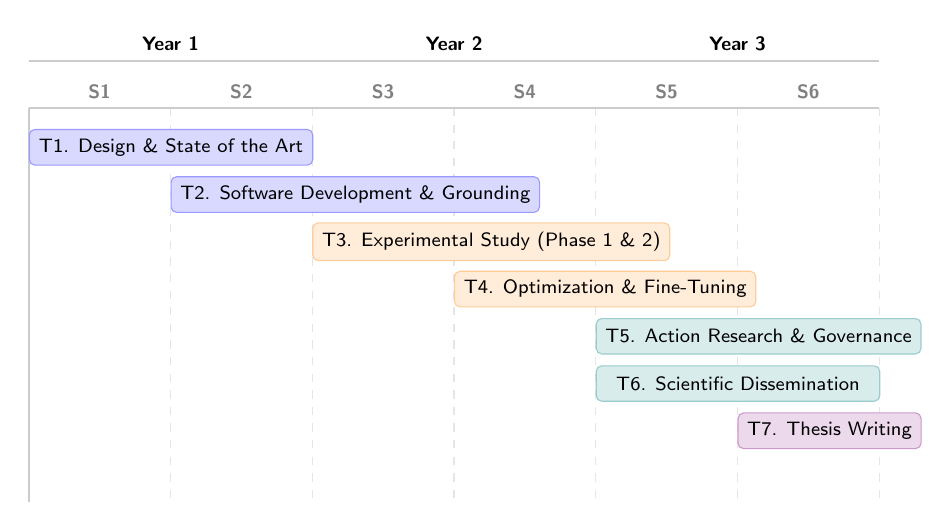
\begin{tikzpicture}[
        task/.style={rectangle, rounded corners=2pt, minimum height=0.45cm, align=left, font=\scriptsize\sffamily, text=black},
        y_axis/.style={draw, -{Latex[scale=0.8]}, thick, gray!70},
        grid_line/.style={draw, gray!20, thin, dashed}
    ]
        % Time Grid Columns (S1 to S6)
        \foreach \x/\label in {1/S1, 2/S2, 3/S3, 4/S4, 5/S5, 6/S6} {
            \draw[grid_line] (\x*1.8, 0.5) -- (\x*1.8, -4.5);
            \node[font=\scriptsize\sffamily\bfseries, gray] at (\x*1.8 - 0.9, 0.7) {\label};
        }
        % Years headers
        \draw[draw=gray!40, thick] (0, 1.1) -- (3.6, 1.1) node[midway, above, font=\scriptsize\sffamily\bfseries] {Year 1};
        \draw[draw=gray!40, thick] (3.6, 1.1) -- (7.2, 1.1) node[midway, above, font=\scriptsize\sffamily\bfseries] {Year 2};
        \draw[draw=gray!40, thick] (7.2, 1.1) -- (10.8, 1.1) node[midway, above, font=\scriptsize\sffamily\bfseries] {Year 3};
        
        % Y-axis (Tasks labels border/separator)
        \draw[draw=gray!40, thick] (0, 0.5) -- (10.8, 0.5);
        \draw[draw=gray!40, thick] (0, 0.5) -- (0, -4.5);
        
        % Task bars (X start, Width, Y pos, Color, Text)
        % Year 1
        \node[task, fill=blue!15, draw=blue!40, minimum width=3.6cm, anchor=west] at (0, 0) {T1. Design \& State of the Art};
        \node[task, fill=blue!15, draw=blue!40, minimum width=3.6cm, anchor=west] at (1.8, -0.6) {T2. Software Development \& Grounding};
        
        % Year 2
        \node[task, fill=orange!15, draw=orange!40, minimum width=3.6cm, anchor=west] at (3.6, -1.2) {T3. Experimental Study (Phase 1 \& 2)};
        \node[task, fill=orange!15, draw=orange!40, minimum width=3.6cm, anchor=west] at (5.4, -1.8) {T4. Optimization \& Fine-Tuning};
        
        % Year 3
        \node[task, fill=teal!15, draw=teal!40, minimum width=3.6cm, anchor=west] at (7.2, -2.4) {T5. Action Research \& Governance};
        \node[task, fill=teal!15, draw=teal!40, minimum width=3.6cm, anchor=west] at (7.2, -3.0) {T6. Scientific Dissemination};
        \node[task, fill=violet!15, draw=violet!40, minimum width=1.8cm, anchor=west] at (9.0, -3.6) {T7. Thesis Writing};
        
    \end{tikzpicture}
    \caption{Three-year Gantt chart of the research activities.}
    \label{fig:gantt}
\end{figure}

\newpage

% ------------------------------------------------------------------------------
% 5) EXPECTED RESULTS
% ------------------------------------------------------------------------------
\section{Expected results}

The research aims to produce concrete results for clinical practice and service management:
\begin{enumerate}
    \item \textbf{Evidence on differential reasoning:} Empirical evaluation of whether support broadens plausible alternatives, makes uncertainty explicit, and reduces omissions, unsupported assumptions, and premature closure.
    \item \textbf{Validation of Digital Anamnesis:} Definition and initial validation of a digital anamnesis sheet, usable by clinicians to understand the impact of commercial chatbot use on patient well-being.
    \item \textbf{Care Governance and Sustainability Model:} Definition of guidelines and risk matrices for the safe adoption of AI in healthcare services, promoting more effective, consistent, and economically sustainable therapeutic pathways.
    \item \textbf{Clinical error reduction:} Estimate between-condition differences in differential-diagnosis quality and reasoning errors.
    \item \textbf{Scientific dissemination:} Publication of at least 3 articles in indexed scientific journals (e.g., \textit{JMIR}, \textit{Frontiers}) and presentations at national and international congresses.
\end{enumerate}

% ------------------------------------------------------------------------------
% 6) PROJECT INNOVATIVENESS
% ------------------------------------------------------------------------------
\section{Project innovativeness}

The project's innovativeness lies in the integration of computer engineering, psychopathology, and clinical governance. The goal is not to introduce AI as a decision shortcut, but to design a controlled environment where technology helps professionals see better, document better, and decide with greater awareness.

\subsection{Engineering Innovation and Edge-Cloud Hybrid Architecture}

Most e-health applications rely on cloud APIs, raising serious concerns regarding health data privacy (GDPR, EU AI Act). This project stands out by implementing a resource-constrained hybrid architecture (\textit{pervasive AI}; Pecori, 2023). Optimizing local execution while establishing a secure, audited cloud fallback for clinical inference---alongside offloading non-sensitive training tasks---represents a technical innovation that guarantees both legal and economic sustainability for digital health services.

\subsection{Epistemological Innovation and Nosographical Grounding}

Unlike standard ML approaches treating LLMs as predictive black boxes, the project introduces a theoretical-technical innovation grounded in the ``epistemology of simulation'' (Vidotto, Ditolve \& Panzeri, 2026). Since LLMs simulate cognitive activity without real semantic comprehension, the system is designed to serve as a ``cognitive mirror'' but to function as critical support and a nosographical organizer. This approach protects phenomenological diagnosis (Jaspers, 1963) and maintains clinical responsibility with the human professional.

\subsection{Relational Innovation: Digital Anamnesis in the Clinical Setting}

The project is innovative in defining and validating a formal \textit{Digital Anamnesis} protocol to address patients' spontaneous use of commercial chatbots. By viewing conversational AI as a ``new relational and transitional object'' (Cremaschi \& Pierotti, 2026), this research provides therapists with structured tools to map and address dysfunctional interaction patterns (cybercondria, isolation), preventing therapeutic alliance deterioration.

\subsection{Interdisciplinary Synergy for Care Sustainability}

The project represents a concrete convergence between clinical psychology/psychometrics (research lines 4 and 5) and computer engineering (SSD IINF-05/A). Care sustainability is redefined as care quality sustainability: computer engineering provides the secure, optimized infrastructure that reduces diagnostic error and cognitive load, enabling personalized clinical pathways that safeguard patient well-being.

% ------------------------------------------------------------------------------
% 7) ESSENTIAL BIBLIOGRAPHY
% ------------------------------------------------------------------------------
\section{Essential bibliography}

\begin{enumerate}[label={[\arabic*]}]
    \item Bordin, E. S. (1979). The generalizability of the psychoanalytic concept of the working alliance. \textit{Psychotherapy: Theory, Research \& Practice}, 16(3), 252. \url{https://doi.org/10.1037/h0085885}
    \item Cremaschi, M., \& Pierotti, A. P. (2026). Intelligenza artificiale in psicopatologia: Epistemologia clinica, relazione terapeutica e governance. Manuscript submitted for publication.
    \item Cremaschi, M., \textbf{Ditolve, D.}, Curcio, C., Panzeri, A., Spoto, A., \& Maurino, A. (2025). Decoding the mind: A RAG-LLM on ICD-11 for decision support in psychology. \textit{Expert Systems with Applications}, 279, 127191. \url{https://doi.org/10.1016/j.eswa.2025.127191}
    \item Dohnány, S., Kurth-Nelson, Z., et al. (2026). Technological folie à deux: Feedback loops between AI chatbots and mental illness. \textit{Nature Mental Health}. Advance online publication. \url{https://doi.org/10.1038/s44220-026-00595-8}
    \item Finn, S. E. (2007). In our clients' shoes: Theory and techniques of therapeutic assessment. \textit{Lawrence Erlbaum Associates}. \url{https://doi.org/10.4324/9781003064459}
    \item Flückiger, C., Del Re, A. C., \& Horvath, A. O. (2018). The alliance in adult psychotherapy: A meta-analytic synthesis. \textit{Psychotherapy}, 55(4), 316--340. \url{https://doi.org/10.1037/pst0000172}
    \item Jaspers, K. (1963). \textit{General psychopathology}. University of Chicago Press.
    \item Kendler, K. S. (2016). The nature of psychiatric disorders. \textit{World Psychiatry}, 15(1), 5--12. \url{https://doi.org/10.1002/wps.20292}
    \item Parnas, J., Sass, L. A., \& Zahavi, D. (2013). Rediscovering psychopathology: The epistemology and phenomenology of the psychiatric object. \textit{Schizophrenia Bulletin}, 39(2), 270--277. \url{https://doi.org/10.1093/schbul/sbs153}
    \item Pecori, R. (2023). Pervasive and resource-constrained AI in healthcare: Applications in e-health and CDSS. In \textit{Proc. PeRConAI Workshop}.
    \item Sharma, M., et al. (2023). Towards understanding sycophancy in language models. \textit{arXiv}. \url{https://arxiv.org/abs/2310.13548}
    \item Stanghellini, G., \& Fuchs, T. (Eds.). (2013). \textit{One century of Karl Jaspers' general psychopathology}. Oxford University Press. \url{https://doi.org/10.1093/med/9780199609253.001.0001}
    \item Vidotto, G., \textbf{Ditolve, D.}, \& Panzeri, A. (2026). Una riflessione critica sui Large Language Models in psicologia clinica: Malfunzionamento, metacognizione, memoria ed etica. \textit{Psicoterapia Cognitiva e Comportamentale}, 32(2). \url{https://doi.org/10.14605/PCC3222605}
    \item World Health Organization. (2024). Ethics and governance of AI for health: Guidance on large multi-modal models. \textit{WHO}. \url{https://www.who.int/publications/i/item/9789240084759}
\end{enumerate}

\end{document}